%\section[Fundamental Concepts]{\hyperlink{toc}{Fundamental Concepts}}
\section{Fundamentals}

Complex numbers can be thought as an extension to the real number system in which we have a solution for the $x^2 +1 = 0 $ equation. There are some mathematically rigorous ways to construct the complex numbers from real numbers. However, those mathematically rigorous ways came out only recently (20th century) and there were not around when the first ideas of complex numbers were forming around 18th century.  For that reason I have not discussed the detailed mathematical construction of the complex numbers here. \\

As discussed earlier, complex numbers system is a system in which we have a solution for the $x^2+1=0$ equation which is represented as $i = \sqrt{-1}$. A complex number is written like $z = a+bi$ in which $a,b \in \mathbb{R}$ and the set of all complex numbers is denoted as $\mathbb{C}$. It is easy to check that complex numbers still satisfy the \emph{commutative}, \emph{associative}, and \emph{distributive} properties similar to the real numbers. \\

\begin{defbox}{Set of Complex Numbers and Basic Definitions $\mathbb{C}$}

	\begin{itemize}
		\item The set of complex numbers: The set of complex numbers $\mathbb{C}$ is:
		
		\[ \mathbb{C} = \{ z = a+bi : a,b \in \mathbb{R}, i = \sqrt{-1} \} \]
		
		In which we call $a$ as the \emph{real part} and $b$ as the \emph{complex part} of the complex number $z$ and we show that as: 
		
		\begin{align*}
			\Re(z) = a \\
			\Im(z) = b
		\end{align*}
		
		
		
		\hrule
		
		\item Two complex numbers $z_1 = a_1 + b_1 i$ and  $z_2 = a_2 + b_2 i$ are equal if:
		
		\begin{align*}
			\Im(z_1) = \Im (z_2) \\
			\Re(z_1) = \Re (z_2) 
		\end{align*}
		
		\hrule
		
		\item Polar representation of the complex numbers: A complex number $z = a+bi$ can be written as:
		
		\[ z = r e^{i\phi} \]
		
		in which $r$ is the modulus of $z$ and $\phi$ is the argument of $z$ which is defined as: $\phi = \arctan(\frac{a}{b})$. Also we define the set $Arg$ as:
		
		\[ Arg(z) = \{ arg(z)+2\pi n : n \in \mathbb{Z} \}\]
		
		\hrule
		
		\item Complex conjugate: The complex conjugate of a complex number $z = a + bi$ is defined as: \[ \overline{z} = a - bi \]
		
		\hrule
		
		\item Modulus of a complex number: The modulus of a complex number $z = a + bi$ is defined as:\
		\[ |z| = \sqrt{z \overline{z}} = \sqrt{a^2 + b^2}\]
	
	\end{itemize}

\end{defbox}

The following figure summarizes the basic properties of the complex numbers discussed above. \\

\begin{figure}
	\centering
	\begin{tikzpicture}[scale=2]
	  \def\xmax{2.0}
	  \def\ymax{1.6}
	  \def\R{1.9}
	  \def\ang{35}
	  \coordinate (O) at (0,0);
	  \coordinate (R) at (\ang:\R);
	  \coordinate (-R) at (-\ang:\R);
	  \coordinate (X) at ({\R*cos(\ang)},0);
	  \coordinate (Y) at (0,{\R*sin(\ang)});
	  \coordinate (-Y) at (0,{-\R*sin(\ang)});
	  \node[fill=mydarkblue,circle,inner sep=0.8] (point) at (R) {};
	  \node[fill=mydarkred,circle,inner sep=0.8] (-point) at (-R) {};
	  \node[mydarkblue,above right=-2] at (R) {$z=x+iy=re^{i\theta}$};
	  \node[mydarkred,below right=-1] at (-R) {$\overline{z}=x-iy=re^{-i\theta}$};
	  \draw[dashed,mydarkblue] (Y) -- (point) -- ++ (0,{0.1-\R*sin(\ang)});
	  \draw[dashed,mydarkred](-Y) -- (-point) --++ (0,{\R*sin(\ang)-0.45});
	  \draw[->,line width=0.9] (-0.55*\xmax,0) -- (\xmax+0.05,0) node[right] {Re};
	  \draw[->,line width=0.9] (0,-\ymax) -- (0,\ymax+0.05) node[left] {Im};
	  \draw[vector] (O) -- (point) node[pos=0.55,above left=-2] {$r$};
	  \draw[vector,myred] (O) -- (-point) node[pos=0.55,below left=-2] {$r$};
	  \draw pic[->,"$\theta$",mydarkblue,draw=mydarkblue,angle radius=23,angle eccentricity=1.24]
	    {angle = X--O--R};
	  \draw pic[<-,"$-\theta$"{right=-1},mydarkred,draw=mydarkred,angle radius=20,angle eccentricity=1]
	    {angle = -R--O--X};
	  %\tick{X}{90} node[scale=0.9,left=6,below right=-2] {$x = r\cos\theta$};
	  \tick{X}{90} node[scale=1,below=-1] {$x$};
	  \tick{Y}{ 0} node[mydarkblue,scale=1,left] {$y$}; %r\sin\theta = 
	  \tick{-Y}{ 0} node[mydarkred,scale=1,left] {$-y$};
	\end{tikzpicture}
	\caption{A summary of the polar and Cartesian representation of the complex numbers.}
\end{figure}



\begin{propbox}{Fundamental Properties of Complex Numbers}
	Using the definition of the complex numbers, we can show that they satisfy the following properties. \\
	
	\begin{enumerate}
	
		\item Commutative property for the sum and product: 
		\begin{gather}
		a + b = b + a \\
		ab = ba
		\end{gather}
		
		\item Associative property for the sum and product
		\begin{gather}
		a + (b+c) = (a+b) + c \\
		a(bc) = (ab)c
		\end{gather}
		
		\item Distributive property:
		\begin{gather}
		a (b+c) = ab + ac
		\end{gather}
	
	\end{enumerate}
\end{propbox}

\begin{proof}
	All of the statements can be proved by writing complex numbers as $z = x+yi$ and substituting in the equations.
\end{proof}

Utilizing the basic definitions along with the mathematical logic, we can derive different properties for complex numbers. The following properties come in handy when solving problems:

\begin{propbox}{Basic Properties of Complex Numbers}
	
	\begin{gather}
	\conj{z_1 + z_2} = \conj{z_1} + \conj{z_2} \\
	\conj{z_1 z_2} = \conj{z_1} \conj{z_2} \\
	\conj{(\frac{z_1}{z_2})} = \frac{\conj{z_1}}{\conj{z_2}}  \\
	\conj{(\conj{z})} = z \\
	\Re(z) = \frac{z + \conj{z}}{2} \\
	\Im(z) = \frac{z - \conj{z}}{2i} \\
	(\conj{z})^k = \conj{(z^k)} \\  
	|z_1 z_2| = |z_1||z_2|
	\end{gather}

\end{propbox}

\begin{proof}
	The proof for some of the properties: \\
	\begin{itemize}
	\item $|z_1 z_2|= |z_1||z_2|$: To show this we first need to raise the both sides to the power 2:
	\[ |z_1 z_2|^2 = (z_1 z_2)\conj{(z_1 z_2)} = (z_1 \conj{z_1})(z_2 \conj{z_2}) = |z_1|^2|z_2|^2 \]. So by taking the square root of the both sides we will arrive at: $|z_1 z_2| = |z_1||z_2|$
	
	\item $(\conj{z})^k = \conj{(z^k)}$: Let's start from the right hand side:
	
	\[ \conj{(z^k)} = \conj{(\underbrace{z*z*z*\ldots*z}_\text{k times})} = \underbrace{\conj{z}*\conj{z}*\conj{z}*\ldots*\conj{z}}_\text{k times} = (\conj{z})^k\]
	\end{itemize}
\end{proof}


\begin{example}{Ordering Property in Complex Numbers}
	\emph{Question.} Show that we can not define any ordering property in the complex numbers.
	\begin{proof}
		Suppose that we \emph{can} define ordering property in the complex numbers. So two cases might arise for the $i$. It will be $i>0$ or $i<0$. 
		
		\begin{itemize}
		\item Let's assume that $i>0$. Since $f(x) = x^2$ is a strictly increasing function, then by arising two sides of the inequality to the power of two we will have: $i^2 = -1 > 0$ which is a contradiction.
		
		\item Let's assume that $i<0$. Since $i$ is smaller than zero, we can multiply the two sides of the inequality by $i$ but we should change the direction of the inequality sign. So we will have $i*i = -1 > 0$ which again arises a mathematical contradiction.
		\end{itemize}
		
		So we can conclude that we can not have any ordering property in the set of complex numbers.
	\end{proof}
\end{example}



We can also have some important inequalities in the complex numbers that often come very handy in solving problems. The following box summarizes some of them.


 
\begin{thmbox}{Important Inequalities in Complex Numbers}

	\begin{enumerate}
		\item Basic Inequalities
		\begin{align*}
			\Re(z) \leq |z| \\
			\Im(z) \leq |z|
		\end{align*}
		
		\item Triangle Inequality \[ |z_1 + z_2| \leq |z_1| + |z_2| \]
	\end{enumerate}

\end{thmbox}

\begin{proof}
	\ \\
	\begin{itemize}
	\item Triangle Inequality (proof number 1): Let's start by raising the right hand side to the power 2 and simplify the equation:
	
	\[ |z_1 + z_2|^2 = (z_1 + z_2) \conj{(z_1 + z_2)} = z_1 \conj{z_1} + z_2 \conj{z_2} + z_1 \conj{z_2} + \conj{z_1} z_2 \]
	
	\end{itemize}
\end{proof}


\begin{example}{Cyclic Property of $i$}
	By using the basic property of the complex number $i = \sqrt{-1}$, for every $k \in \mathbb{Z}$ we can show that:
	
	\begin{align*}
		i^{4k} &= 1 \\
		i^{4k+1} &= i \\
		i^{4k+2} &= -1 \\
		i^{4k+3} &= -i
	\end{align*}
	This also represent that fact that multiplying a complex number by $i$ means a $\pi/2$ counterclockwise rotation. This becomes very clear if we consider the polar representation of complex numbers.
	

	\centering
	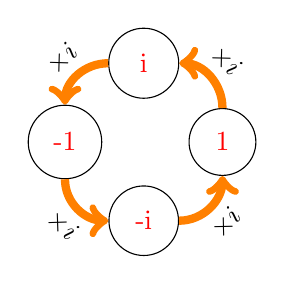
\begin{tikzpicture}[inner sep=4mm]
		%		\draw [step=0.5, gray!50!white, line width=0.1] (-2,-2) grid (2,2);
		\node[red, circle, draw=black,inner sep=0.2cm] (1) at (1,0) {1};
		\node[red, circle, draw=black,inner sep=0.23cm] (i) at (0,1) {i};
		\node[red, circle, draw=black,inner sep=0.2cm] (-1) at (-1,0) {-1};
		\node[red, circle, draw=black,inner sep=0.2cm] (-i) at (0,-1) {-i};
		\draw[->, orange, line width=3] (1) to[out=90, in=0] node[sloped, black, anchor=south,inner sep=1mm] {$\times i$} (i);
		\draw[->, orange, line width=3] (i) to[out=-180, in=90] node[sloped, black, anchor=south,inner sep=1mm] {$\times i$} (-1);
		\draw[->, orange, line width=3] (-1) to[out=-90, in=180] node[sloped, black, anchor=north,inner sep=1mm] {$\times i$} (-i);
		\draw[->, orange, line width=3] (-i) to[out=0, in=-90] node[sloped, black, anchor=north,inner sep=1mm] {$\times i$} (1);									;
		
		
	\end{tikzpicture}



\end{example}



\begin{example}{Karatsuba Algorithm}
	Suppose that we want to multiply two complex numbers $z_1 = a + bi$ and $ z_2 = c + di$ in the computer and return $z = z_1 + z_2$. To do that we should get the imaginary and real part of two numbers and then return:
	
	\begin{align*}
		\Re (z) &= ac - bd \\
		\Im (z) &= bc + ad
	\end{align*}
	
	So to multiply two complex numbers in the computer, we need to do 4 multiplications and 2 additions. So performing multiplication takes considerably more clock cycles in CPU. However we can do a trick to reduce the number of multiplications to 3 with a cost of some extra additions. To do so we need to calculate three intermediate variables each of which require one multiplication.
	
	\begin{align*}
		t_1 &= ac \\
		t_2 &= bd \\
		t_3 &= (a+b)(c+d)
	\end{align*}
	
	So we will have:
	
	\begin{align*}
		\Re (z) &= t_1 - t_2 \\
		\Im (z) &= t_3 - (t_1 + t_2)
	\end{align*}
	
	So using the Karatsuba algorithm we will have 3 multiplications, and 5 addictions. There is a very interesting story behind this discovery by the Karatsuba in 1960 (when he was a 23-year-old graduate student) that he somehow proved the Kolmogorov's statement is wrong! You can read more on this in the Wikipedia page of Karatsuba algorithm.   
\end{example}

\begin{example}{Complex Roots}
	Find all of the roots of the following equations
	
	\begin{enumerate}
		\item $z^4 -16 = 0$
		\begin{sol}
			Writing the complex number in the form of its polar representation will ease finding the roots of this equation significantly. So let's assume \[ z = r e^{i\phi} \]
			Then by substituting in the equation we will have:
			\begin{align*}
			r^4 e^{4i\phi} = 16 = 16 e^{2n\pi i}
			\end{align*}
			
			So we will have: $r = 2$ and $\phi = \{ n \pi /2: n \in \mathbb{R} \} = \{ 0, \pi/2, \pi, 3\pi/2 \}$.
		\end{sol}
		\item $\frac{z}{1-z} = 1-5i$
		\begin{sol}
			\begin{flalign*}
				z  & = (1-z)(1-5i) \\
				& = 1-5i - z - 5iz \\
				& = \frac{1-5i}{2-5i} = \frac{(1-5i)(2+5i)}{29}
		\end{flalign*}
		
		\end{sol}
	\end{enumerate}
\end{example}

\begin{propbox}{Roots of Polynomial}
	if $z_0$ is the root of the following polynomial equation (in which $a_i \in \mathbb{R}$):
	
	\[ z^n + a_1 z^{n-1} + a_2 z^{n-2} + \ldots + a_n = 0 \]
	
	then $\conj{z_0}$ is also the root of the equation.

\end{propbox}

\begin{proof}
	This can easily be shown by taking the complex conjugate from both sides of the equation, and then using the fact that $(\conj{z})^k = \conj{(z^k)}$.

\end{proof}


\begin{example}{Matrices with Complex Entries}
	TO BE COMPLETED

\end{example}


\section{Planar Sets and Geometry}
The interesting fact about the complex plane that I like the most is that we can construct different good looking (!) sets in the complex plain $\mathbb{C}$ with quite simple statements. For example the inequality $ |z| \leq 9 $ represents a circle in the complex plane centred at the origin and has a radius of 3. \\

\begin{figure}[h!]
	\centering
	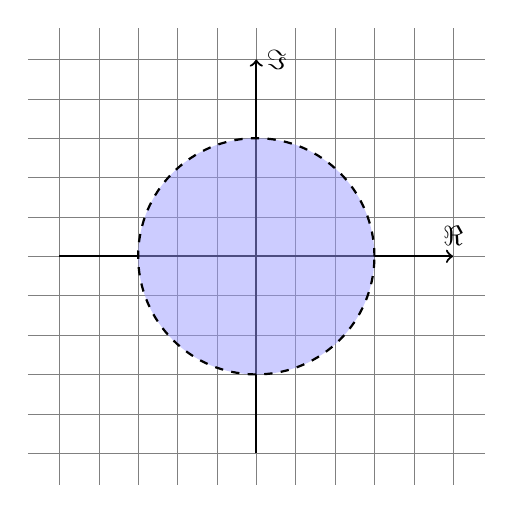
\begin{tikzpicture}
		\draw[step=0.5, black!10!white, help lines](-2.9,-2.9) grid (2.9, 2.9);
		\draw[thick, ->] (-2.5,0) -- (2.5,0) node[anchor=south] {$\Re$};
		\draw[thick, ->] (0,-2.5) -- (0,2.5) node[anchor=west]{$\Im$};
		\filldraw[blue!40!white, thick, dashed, draw=black, fill opacity=0.5] (0,0) circle (1.5cm);
	\end{tikzpicture}
	\caption{The planar set representing $ |z| \le 3 $}
\end{figure}



\begin{example}{}
	\emph{Question.} Derive the points in $\mathbb{C}$ that satisfy following conditions.
	
	\begin{enumerate}
		\item $|z+2| = |z-1|$ \\
		\emph{Solution.} There is not a single method that works the best for all of the problems. For this question, it is better to raise both sides of the eqution to the power 2.
		\begin{align*}
			|z+2|^2 &= |z-1|^2 \\
			(z+2)\conj{(z+2)} &= (z-1) \conj{(z-1)} \\
			(z+2)(\conj{z} + 2) &= (z-1) (\conj{z} - 1) \\
			z \conj{z} + 2z + 2\conj{z} + 4 &= z \conj{z} - z - \conj{z} + 1 \\ 
			z + 1 &= - \conj{z}
		\end{align*}
		So let's assume $z$ is in the form $z = x + iy$. By inserting this in equation above we will get:
		\begin{align*}
			(x+1) + iy = -x + iy
		\end{align*}
		So:
		\begin{align*}
			x &= \frac{1}{2}\\
			y &= \text{any real number}
		\end{align*}
		
		So the set of points satisfying this equation will be: \\ \\
		\begin{center}
			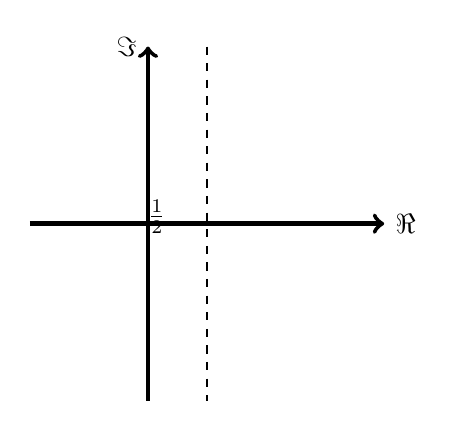
\begin{tikzpicture}[scale=1.5]
				\draw[->, ultra thick] (-1,0) -- (2,0) node [right] {$\Re$};
				\draw[->, ultra thick] (0,-1.5) -- (0,1.5) node [left] {$\Im$};
				\draw[thick, dashed] (0.5,1.5) -- (0.5,-1.5);
				\tick{0.5,0}{90} node[scale=1,below,fill=gray!15] {$\frac{1}{2}$};
			\end{tikzpicture}
		\end{center}
	
		\hrule
		
		\item $|z-1| = \Re{z} + 1$ \\
		\emph{Solution. } For this question it is better to start with a general form of $z = x + iy$ and then substitute in the equation.
		
		\begin{align*}
			|(x-1) + yi| &= x+1 \\
			(x-1)^2 + y^2 &= (x+1)^2 \\
			z^2 - 2x + 1 + y^2 &= x^2 + 2x + 1 \\
			y^2 &= 4x
		\end{align*}
		So the points of complex plain that satisfy the equation will be like the curve:
		\begin{center}
			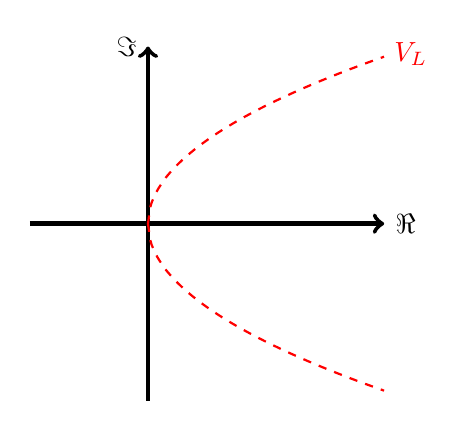
\begin{tikzpicture}[scale=1.5]
				\draw [->, ultra thick] (-1,0) -- (2,0) node [right] {$\Re$};
				\draw [->, ultra thick] (0,-1.5) -- (0,1.5) node [left] {$\Im$};
				\draw[thick,samples=100,smooth,variable=\x,domain=0:2,red, dashed]
				plot(\x,{(\x)^0.5}) node[above=1,right] {$V_L$}
				plot(\x,{-(\x)^0.5});
			\end{tikzpicture}
		\end{center}
	\end{enumerate}
	




\end{example}




\section{Complex Maps}

\subsection{Linear Map}

\subsection{Inverse Map}

\subsection{Mobius Map}

\subsection{Quadratic Map}

\subsection{Exponential Map}


\section{Calculus for Complex variables}

\subsection{Limit}

\subsection{Continuity}

\subsection{Differentiability}
